\documentclass[tikz]{standalone}
\usepackage{tikz}

\usepackage[fontsize=14pt]{fontsize}

\usetikzlibrary{matrix,positioning,shapes.arrows,fit}

\tikzset{ 
table/.style={
  matrix of nodes,
  row sep=-\pgflinewidth,
  column sep=-\pgflinewidth,
  nodes={
    rectangle,draw,
    text width=0.5cm,
    %minimum width=0.75cm,
    %minimum height=0.75cm,
    align=center},
  text depth=0.125cm,
  text height=0.25cm,
  nodes in empty cells,
  outer sep=0cm,
  },
%texto/.style={font=\footnotesize\sffamily},
%title/.style={font=\small\sffamily}
}

\begin{document}
    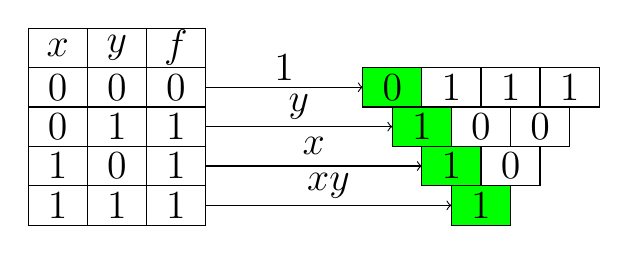
\begin{tikzpicture}[
            every node/.style = {
                draw, rectangle, 
                minimum width=0.75cm,
                minimum height=0.5cm,
                outer sep=0cm, inner sep=0cm,
                node distance=0cm
            }
        ]
        \node (x) {$x$};
        \node [right=of x.east] (y) {$y$};
        \node [right=of y.east] (f) {$f$};

        \node [below=of x.south] (x0) {$0$};
        \node [below=of x0.south] (x1) {$0$};
        \node [below=of x1.south] (x2) {$1$};
        \node [below=of x2.south] (x3) {$1$};

        \node [below=of y.south] (y0) {$0$};
        \node [below=of y0.south] (y1) {$1$};
        \node [below=of y1.south] (y2) {$0$};
        \node [below=of y2.south] (y3) {$1$};
        
        \node [below=of f.south] (f0) {$0$};
        \node [below=of f0.south] (f1) {$1$};
        \node [below=of f1.south] (f2) {$1$};
        \node [below=of f2.south] (f3) {$1$};

        \node [right=2cm of f0.east, fill=green] (r00) {0};
        \node [right=of r00.east] (r01) {1};
        \node [right=of r01.east] (r02) {1};
        \node [right=of r02.east] (r03) {1};

        \node [below=of r00.south east, fill=green] (r10) {1};
        \node [right=of r10.east] (r11) {0};
        \node [right=of r11.east] (r12) {0};

        \node [below=of r10.south east, fill=green] (r20) {1};
        \node [right=of r20.east] (r21) {0};

        \node [below=of r20.south east, fill=green] (r30) {1};

        \draw [->] (f0.east) -- node[draw=none, above] {1} (r00.west);
        \draw [->] (f1.east) -- node[draw=none, above] {$y$} (r10.west);
        \draw [->] (f2.east) -- node[draw=none, above] {$x$} (r20.west);
        \draw [->] (f3.east) -- node[draw=none, above] {$xy$} (r30.west);
    \end{tikzpicture}

    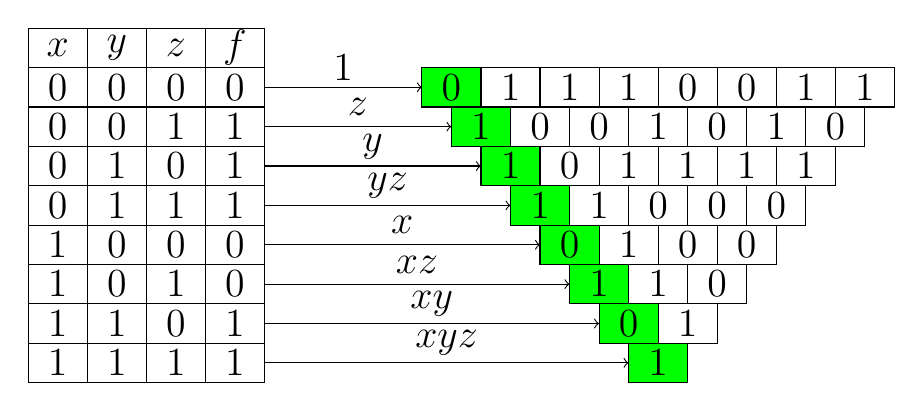
\begin{tikzpicture}[
            every node/.style = {
                draw, rectangle, 
                minimum width=0.75cm,
                minimum height=0.5cm,
                outer sep=0cm, inner sep=0cm,
                node distance=0cm
            }
        ]
        \node (x) {$x$};
        \node [right=of x.east] (y) {$y$};
        \node [right=of y.east] (z) {$z$};
        \node [right=of z.east] (f) {$f$};

        \node [below=of x.south] (x0) {$0$};
        \node [below=of x0.south] (x1) {$0$};
        \node [below=of x1.south] (x2) {$0$};
        \node [below=of x2.south] (x3) {$0$};
        \node [below=of x3.south] (x4) {$1$};
        \node [below=of x4.south] (x5) {$1$};
        \node [below=of x5.south] (x6) {$1$};
        \node [below=of x6.south] (x7) {$1$};

        \node [below=of y.south] (y0) {$0$};
        \node [below=of y0.south] (y1) {$0$};
        \node [below=of y1.south] (y2) {$1$};
        \node [below=of y2.south] (y3) {$1$};
        \node [below=of y3.south] (y4) {$0$};
        \node [below=of y4.south] (y5) {$0$};
        \node [below=of y5.south] (y6) {$1$};
        \node [below=of y6.south] (y7) {$1$};

        \node [below=of z.south] (z0) {$0$};
        \node [below=of z0.south] (z1) {$1$};
        \node [below=of z1.south] (z2) {$0$};
        \node [below=of z2.south] (z3) {$1$};
        \node [below=of z3.south] (z4) {$0$};
        \node [below=of z4.south] (z5) {$1$};
        \node [below=of z5.south] (z6) {$0$};
        \node [below=of z6.south] (z7) {$1$};
        
        \node [below=of f.south] (f0) {$0$};
        \node [below=of f0.south] (f1) {$1$};
        \node [below=of f1.south] (f2) {$1$};
        \node [below=of f2.south] (f3) {$1$};
        \node [below=of f3.south] (f4) {$0$};
        \node [below=of f4.south] (f5) {$0$};
        \node [below=of f5.south] (f6) {$1$};
        \node [below=of f6.south] (f7) {$1$};

        \node [right=2cm of f0.east, fill=green] (r00) {0};
        \node [right=of r00.east] (r01) {1};
        \node [right=of r01.east] (r02) {1};
        \node [right=of r02.east] (r03) {1};
        \node [right=of r03.east] (r04) {0};
        \node [right=of r04.east] (r05) {0};
        \node [right=of r05.east] (r06) {1};
        \node [right=of r06.east] (r07) {1};

        \node [below=of r00.south east, fill=green] (r10) {1};
        \node [right=of r10.east] (r11) {0};
        \node [right=of r11.east] (r12) {0};
        \node [right=of r12.east] (r13) {1};
        \node [right=of r13.east] (r14) {0};
        \node [right=of r14.east] (r15) {1};
        \node [right=of r15.east] (r16) {0};

        \node [below=of r10.south east, fill=green] (r20) {1};
        \node [right=of r20.east] (r21) {0};
        \node [right=of r21.east] (r22) {1};
        \node [right=of r22.east] (r23) {1};
        \node [right=of r23.east] (r24) {1};
        \node [right=of r24.east] (r25) {1};

        \node [below=of r20.south east, fill=green] (r30) {1};
        \node [right=of r30.east] (r31) {1};
        \node [right=of r31.east] (r32) {0};
        \node [right=of r32.east] (r33) {0};
        \node [right=of r33.east] (r34) {0};

        \node [below=of r30.south east, fill=green] (r40) {0};
        \node [right=of r40.east] (r41) {1};
        \node [right=of r41.east] (r42) {0};
        \node [right=of r42.east] (r43) {0};

        \node [below=of r40.south east, fill=green] (r50) {1};
        \node [right=of r50.east] (r51) {1};
        \node [right=of r51.east] (r52) {0};

        \node [below=of r50.south east, fill=green] (r60) {0};
        \node [right=of r60.east] (r51) {1};

        \node [below=of r60.south east, fill=green] (r70) {1};

        \draw [->] (f0.east) -- node[draw=none, above] {1} (r00.west);
        \draw [->] (f1.east) -- node[draw=none, above] {$z$} (r10.west);
        \draw [->] (f2.east) -- node[draw=none, above] {$y$} (r20.west);
        \draw [->] (f3.east) -- node[draw=none, above] {$yz$} (r30.west);
        \draw [->] (f4.east) -- node[draw=none, above] {$x$} (r40.west);
        \draw [->] (f5.east) -- node[draw=none, above] {$xz$} (r50.west);
        \draw [->] (f6.east) -- node[draw=none, above] {$xy$} (r60.west);
        \draw [->] (f7.east) -- node[draw=none, above] {$xyz$} (r70.west);
    \end{tikzpicture}

    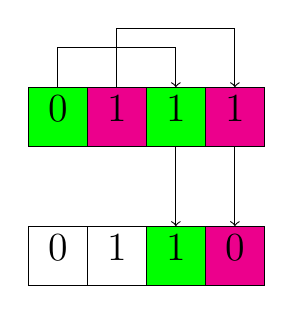
\begin{tikzpicture}[
            every node/.style = {
                %draw, rectangle, 
                minimum width=0.75cm,
                minimum height=0.75cm,
                outer sep=0cm, inner sep=0cm,
                node distance=0cm
            }
        ]
        \matrix [table] (s0)
        {
            \node[fill=green] (s0-1-1) {0}; & 
            \node[fill=magenta] (s0-1-2) {1}; & 
            \node[fill=green] (s0-1-3) {1}; & 
            \node[fill=magenta] (s0-1-4) {1}; \\
        };
        \matrix [table, below=1cm of s0] (s1)
        {
            0 & 1 & 
            \node[fill=green] (s1-1-3) {1}; & 
            \node[fill=magenta] (s1-1-4) {0}; \\
        };
        \draw[->] (s0-1-1.north) -- ++(0,0.5) -| (s0-1-3.north);
        \draw[->] (s0-1-2.north) -- ++(0,0.75) -| (s0-1-4.north);
        \draw[->] (s0-1-3.south) -- (s1-1-3.north);
        \draw[->] (s0-1-4.south) -- (s1-1-4.north);
    \end{tikzpicture}

    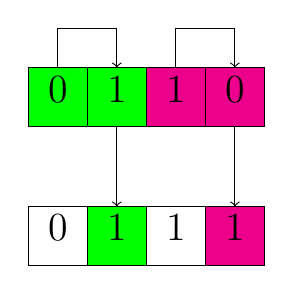
\begin{tikzpicture}[
            every node/.style = {
                %draw, rectangle, 
                minimum width=0.75cm,
                minimum height=0.75cm,
                outer sep=0cm, inner sep=0cm,
                node distance=0cm
            }
        ]
        \matrix [table] (s0)
        {
            \node[fill=green] (s0-1-1) {0}; & 
            \node[fill=green] (s0-1-2) {1}; & 
            \node[fill=magenta] (s0-1-3) {1}; & 
            \node[fill=magenta] (s0-1-4) {0}; \\
        };
        \matrix [table, below=1cm of s0] (s1)
        {
            0 & \node[fill=green] (s1-1-2) {1}; & 
            1 & \node[fill=magenta] (s1-1-4) {1}; \\
        };
        \draw[->] (s0-1-1.north) -- ++(0,0.5) -| (s0-1-2.north);
        \draw[->] (s0-1-3.north) -- ++(0,0.5) -| (s0-1-4.north);
        \draw[->] (s0-1-2.south) -- (s1-1-2.north);
        \draw[->] (s0-1-4.south) -- (s1-1-4.north);
    \end{tikzpicture}
\end{document}